\documentclass[11pt, letterpaper]{article}

\title{ECSE 420 Assignment 1 Report\\Group 19}
\author{
    Stuart Mashaal\\
    \texttt{260639962}
    \and
    Oliver Tse Sakkwun\\
    \texttt{260604362}
}
\date{Due: October 10th, 2018}

\usepackage[utf8]{inputenc} % utf-8 file encoding
\usepackage[margin=0.75in]{geometry} % widen page margins
\usepackage{graphicx} % use external images
\graphicspath{ {images/} } % folder of images
\usepackage{caption}
\setlength\parindent{0pt} % no paragraph indent
\usepackage{amsmath} % math tools
\usepackage{enumitem} % tools for convenient list formatting

\setlength{\jot}{10pt}

\begin{document}

\begin{titlepage}
    \maketitle
    \thispagestyle{empty}
    \setcounter{page}{0}
\end{titlepage}

\section*{Question 1}

\subsection*{1.6}

\begin{figure}[h]
    \centering
    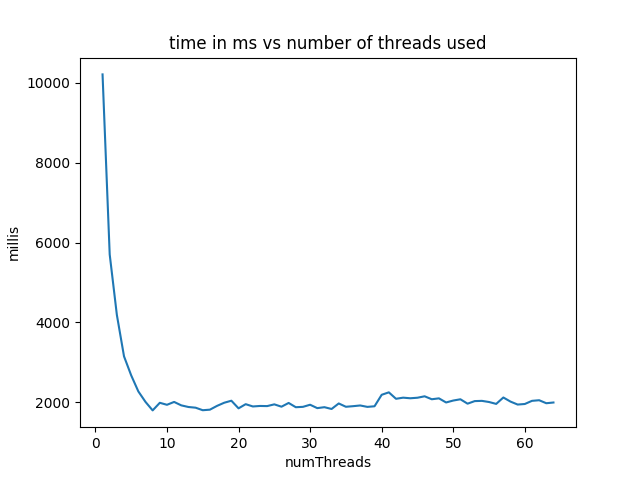
\includegraphics[width=0.5\textwidth]{thread_count_plot.png}
\end{figure}

In the above figure we see that running time drops off sharply (hyperbolic) with the number of
threads until 8 threads. This is sensible since the machine used has 8 cores and Ahmdal's law
predicts that when the entire program is parallelizable, each extra core used increments
the divisor of running time. Once more than 8 threads are used, parallelization is not improved and
each new thread increases (by a small amount each time) the time spent on thread-switching overhead.\\

This explains why the curve appears to rise slowly and monotonically after 8 threads.

\begin{figure}[h]
    \centering
    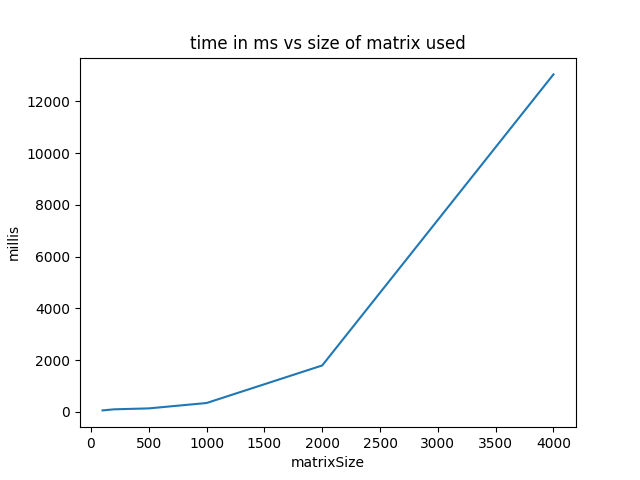
\includegraphics[width=0.5\textwidth]{matrix_size_plot.png}
\end{figure}

The above graphs depicts two function that rise at increasing rates. There is not enough data to
model the functions exactly, but low-order polynomials like $O(n^3)$ are expected since the algorithm
used for matrix multiplication runs in $O(n^3)$. The parallelized algorithm runs in $O(n^3/k)$ where
the constant $k$ is the number of threads, so the graphs above are reasonable since the parallelized
graph looks like it is proportional to the sequential one with a rate of proportionality equal to
$1/k$.

\pagebreak

\section*{Question 2}

\subsection*{2.1}

Deadlock can occur when these four conditions are meet:

\begin{enumerate}
    \item Mutual exclusion: At least one resource must be held in a non-shareable mode. Otherwise, the processes would not be prevented from using the resource when necessary. Only one process can use the resource at any given instant of time
    \item Hold and wait or resource holding: a process is currently holding at least one resource and requesting additional resources which are being held by other processes.
    \item No preemption: a resource can be released only voluntarily by the process holding it.
    \item Circular wait: each process must be waiting for a resource which is being held by another process, which in turn is waiting for the first process to release the resource. In general, there is a set of waiting processes, $P = \{P_1, P_2, ..., P_N\}$, such that $P_1$ is waiting for a resource held by $P_2$, $P_2$ is waiting for a resource held by $P_3$ and so on until $P_N$ is waiting for a resource held by $P_1$.
\end{enumerate}

\subsection*{2.2}

The solution to resolve deadlock is to remove the above conditions by employing the following two strategies:

\begin{enumerate}
    \item Prevention
        \begin{enumerate}[label=\arabic*.]
            \item Mutual exclusion: In general, this condition cannot be disallowed.
            \item Hold-and-wait: The hold and-wait condition can be prevented by requiring that a process request all its required resources at one time, and blocking the process until all requests can be granted simultaneously.
            \item No preemption: One solution is that if a process holding certain resources is denied a further request, that process must release its unused resources and request them again, together with the additional resource.
            \item Circular Wait: The circular wait condition can be prevented by defining a global ordering of resource types. If a process has been allocated resources of type R, then it may subsequently request only those resources of types following R in the ordering.
        \end{enumerate}
    \item Detection and reallocation of resources
        \begin{itemize}
            \item The system constantly monitors processes for deadlocks/unsafe states (for example using the Banker’s Algorithm) and when it detects them, it will restart and/or delays all or some of the offending processes.
        \end{itemize}
\end{enumerate}
\pagebreak

\section*{Question 3}

Deadlock and Starvation in the Dining Philosophers Problem.

\subsection*{3.2}

To avoid deadlock in the Dining Philosophers Problem, we had our philosophers follow two rules:

\begin{enumerate}
	\item A philosopher takes his two chopsticks only if both chopsticks are not in use. Even if all philosophers are hungry simultaneously, only two philosophers can eat, because philosophers must take both chopsticks at once.
same time.
	\item Philosophers on odd numbered take the first left new chopsticks right, while the even-numbered hilosophers take the right chopstick first and chopsticks left. If all philosophers hunger simultaneously, making way for asymmetric solution will prevent all philosophers take the left chopstick simultaneously so that a deadlock condition can be avoided.
\end{enumerate}

\subsection*{3.3}
We use the concept of altruistic philosopher to avoid starvation.If a philosopher picks up a chopstickt and realise that the other one is not available, the later will release it.In a sense,those who are eating will give priority to the philosopher who are waiting to eat and vice versa.When they are both waiting, they will end up alternating.

\pagebreak

\section*{Question 4}

Amdahl's Law:

$$
\text{Speed-Up} = \frac{1}{S + \frac{P}{N}}
$$

where

\begin{itemize}
    \item $S$ and $P$ are the sequential and parallel time percentages of the program, respectively. $S + P = 1$.
    \item $N$ is the number of processors that can be used to paralellize the parallel fraction of the program
\end{itemize}

\subsection*{4.1}

The maximum speed-up of a program occurs when the program is executed on an \textit{infinite} number of processors. So, for a program where the sequential portion is $40\%$ of the program, the maximum speed-up is:

$$
\lim_{N \to \infty}\ {\frac{1}{0.4 + \frac{0.6}{N}}} = \frac{1}{0.4} = 2.5
$$

\subsection*{4.2}

Given a fixed number of processors, $N$, we wish to make a 20\% sequential program twice as fast. We wish to do this by decreasing the program's sequential time percentage, $S$, by a multiplicative factor, $k$. We can find $k$ by isolating it in the following equation:

\begin{alignat*}{2}
            & \quad 0.2 + \frac{0.8}{N}           \quad &&= \quad 2 \cdot \left(0.2 k + \frac{1 - 0.2 k}{N}\right)\\
    \implies& \quad 0.2N + 0.8                    \quad &&= \quad 0.4kN + 2 - 0.4k\\
    \implies& \quad 0.2N - 1.2                    \quad &&= \quad 0.4k \cdot (N - 1)\\
    \implies& \quad \frac{0.2 \cdot (N - 6)}{0.4} \quad &&= \quad k \cdot (N - 1)\\
    \implies& \quad \frac{N - 6}{2 \cdot (N - 1)} \quad &&= \quad k\\
\end{alignat*}

\pagebreak
\subsection*{4.3}

Given a fixed number of processors, $N$, and a program that runs twice as fast when the sequential time percentage, $S$, is divided by 3, the original sequential time percentage found by isolating $S$ in the following equation:

\begin{alignat*}{2}
            & \quad S + \frac{1-S}{N} \quad &&= \quad 2 \cdot \left(\frac{S}{3} + \frac{1-\frac{S}{3}}{N}\right)\\
    \implies& \quad SN - S + 1 \quad        &&= \quad \frac{2SN}{3} + 2 - \frac{2S}{3}\\
    \implies& \quad 3SN - 3S + 3 \quad      &&= \quad 2SN + 6 - 2S\\
    \implies& \quad SN - S \quad            &&= \quad 3\\
    \implies& \quad S \quad                 &&= \quad \frac{3}{N - 1}\\
\end{alignat*}

\end{document}
